\documentclass[
onecolumn,
% hf,
]{ceurart}

\usepackage[linesnumbered, ruled, vlined]{algorithm2e}
\sloppy

\usepackage{listings}
\usepackage{subcaption}
\usepackage{soul}
\usepackage{amsmath}
\usepackage{graphicx}
\usepackage{booktabs}
\usepackage{adjustbox}
\usepackage{float}
\lstset{breaklines=true}

\SetKwProg{class}{CLASS}{}{}
\SetKwProg{method}{METHOD}{}{}

\begin{document}

\copyrightyear{2026}
\copyrightclause{Copyright for this paper by its authors.
  Use permitted under Creative Commons License Attribution 4.0
  International (CC BY 4.0).}

\conference{SSI, project 2025/2026}

\title{A Comparative Study of Audio Feature Extraction and Machine Learning Methods for Bird Species Classification}

\tnotemark[1]

\author[1]{Kryspin Dziarek}[%
email=kd315963@student.polsl.pl
]
\author[1]{Szymon Pająk}[%
email=sp315960@student.polsl.pl
]
\author[1]{Marcin Adamski}[%
email=ma315929@student.polsl.pl
]
\address[1]{Faculty of Applied Mathematics, Silesian University of Technology, Kaszubska 23, 44100 Gliwice, POLAND}

\begin{abstract}
wstep - 1 akapit, co zrobiono, jakie wyniki, minimum 180 słów
\end{abstract}

\begin{keywords}
    Sound analysis\sep Birdsong\sep MFCC (Mel-Frequency Cepstral Coefficients)\sep Random forest\sep Neural network 
\end{keywords}

\maketitle

\section{Introduction}
Audio analysis is a process of examining and measuring sound signals to gain information, it has been a subject of research for many decades\cite{yu2016automatic}, and now, in the age of artificial intelligence, it has many more applications. Machine learning has become an essential tool in audio signal processing, enabling the development of systems capable of analyzing and classifying sounds. Such systems are widely used in applications including speech recognition\cite{zhu2025systematic}, music\cite{serrano2022new} and animal identification\cite{wood2023pairing}, often outperforming human perception of acoustic patterns\cite{spille2018comparing}.
\\\ \\
There are many techniques for feature extraction from sound, one of the most commonly used being Mel-Frequency Cepstral Coefficients (MFCC). This method converts the raw audio signal into a set of coefficients representing the spectral characteristics of sound\cite{abdul2022mel}. Previous studies have established standard configurations for this algorithm, such as the number of Mel filters and cepstral coefficients. However, optimal values depend on specific dataset and application, such as detection of breathing phase\cite{zhantleuova2025optimizing} or respiratory diseases\cite{yan2025optimizing}.
\\\ \\
In addition to sound recognition, various machine learning algorithms have been applied to audio classification tasks, each providing different levels of performance. Simpler algorithms, such as k-nearest neighbors and random forests, are faster, but often less accurate solutions, while the complex ones, like neural networks, provide higher accuracy at the cost of increased computational complexity.
\\\ \\\ \\
This paper presents bird species recognition with sound analysis (using MFCC) and compares different approaches for this system. The sound analysis algorithm consists of many stages, two of them are especially important, because the values they provide depend on chosen data. The number of filters used to describe the frames and number of compressed coefficients strongly affects the performance of the result. Too many features may introduce noise and redundancy, while too few may lead to information loss. The experiments conducted on a common dataset aim to identify the most effective approach for extracting the MFCC features and developing simple classification models with the best performance.










%opis szczegółów, jak działa metodologia, wszystkie wzory

%mile widziany pseudokod w Algorithm2e

%Wizualizacja działania metody - tez może być

\section{Methodology}

This section outlines the approach used to compare different methods of audio feature extraction and the development of machine learning models for identifying bird species.

\subsection{Audio Feature Extraction}

Audio feature extraction enables the transformation of birdsong recordings into numerical representations, which are crucial for training machine learning models. A custom library called \textit{SoundFeatures} was developed to implement the full extraction pipeline. This section describes its structure and role within the experimental setup.

\subsubsection{Audio Format Conversion}

Audio files were converted from MP3 to FLAC format to provide a consistent and lossless compression of the signal. Although this conversion does not restore the data lost during MP3 compression, it eliminates decoding artifacts and ensures stable input for further signal processing \cite{shi2024data}.

\subsubsection{Framing}

Framing process consists of dividing the signal into smaller pieces. The resulting segments overlap to reduce the risk of cutting important parts, which could lead to data loss. The framing algorithm used in class had a default frame size set to 25ms and hop size set to 10ms. The algorithm extracts frames using a sliding window of fixed length across the entire signal. Every step has a constant value equal to hop size.
\\
\begin{algorithm}[H]
  \caption{Framing method}
  \SetAlgoLined
  \class{SoundFeatures}{
    \SetAlgoVlined
    \method{frame\_signal(signal, frame\_size, hop\_size)}{
      frames = []\;
      \For{i in range(0, lenghtOf(signal) - frame\_size, hop\_size)}{
        frames.append(signal[i:i\ +\ frame\_size])\;
      }
      \Return frames\;
    }
    \vdots
  }
\end{algorithm}

\begin{figure}
  \caption{Visual interpretation of signal framing (hop size set to 110ms and frame size set to 330ms)}
  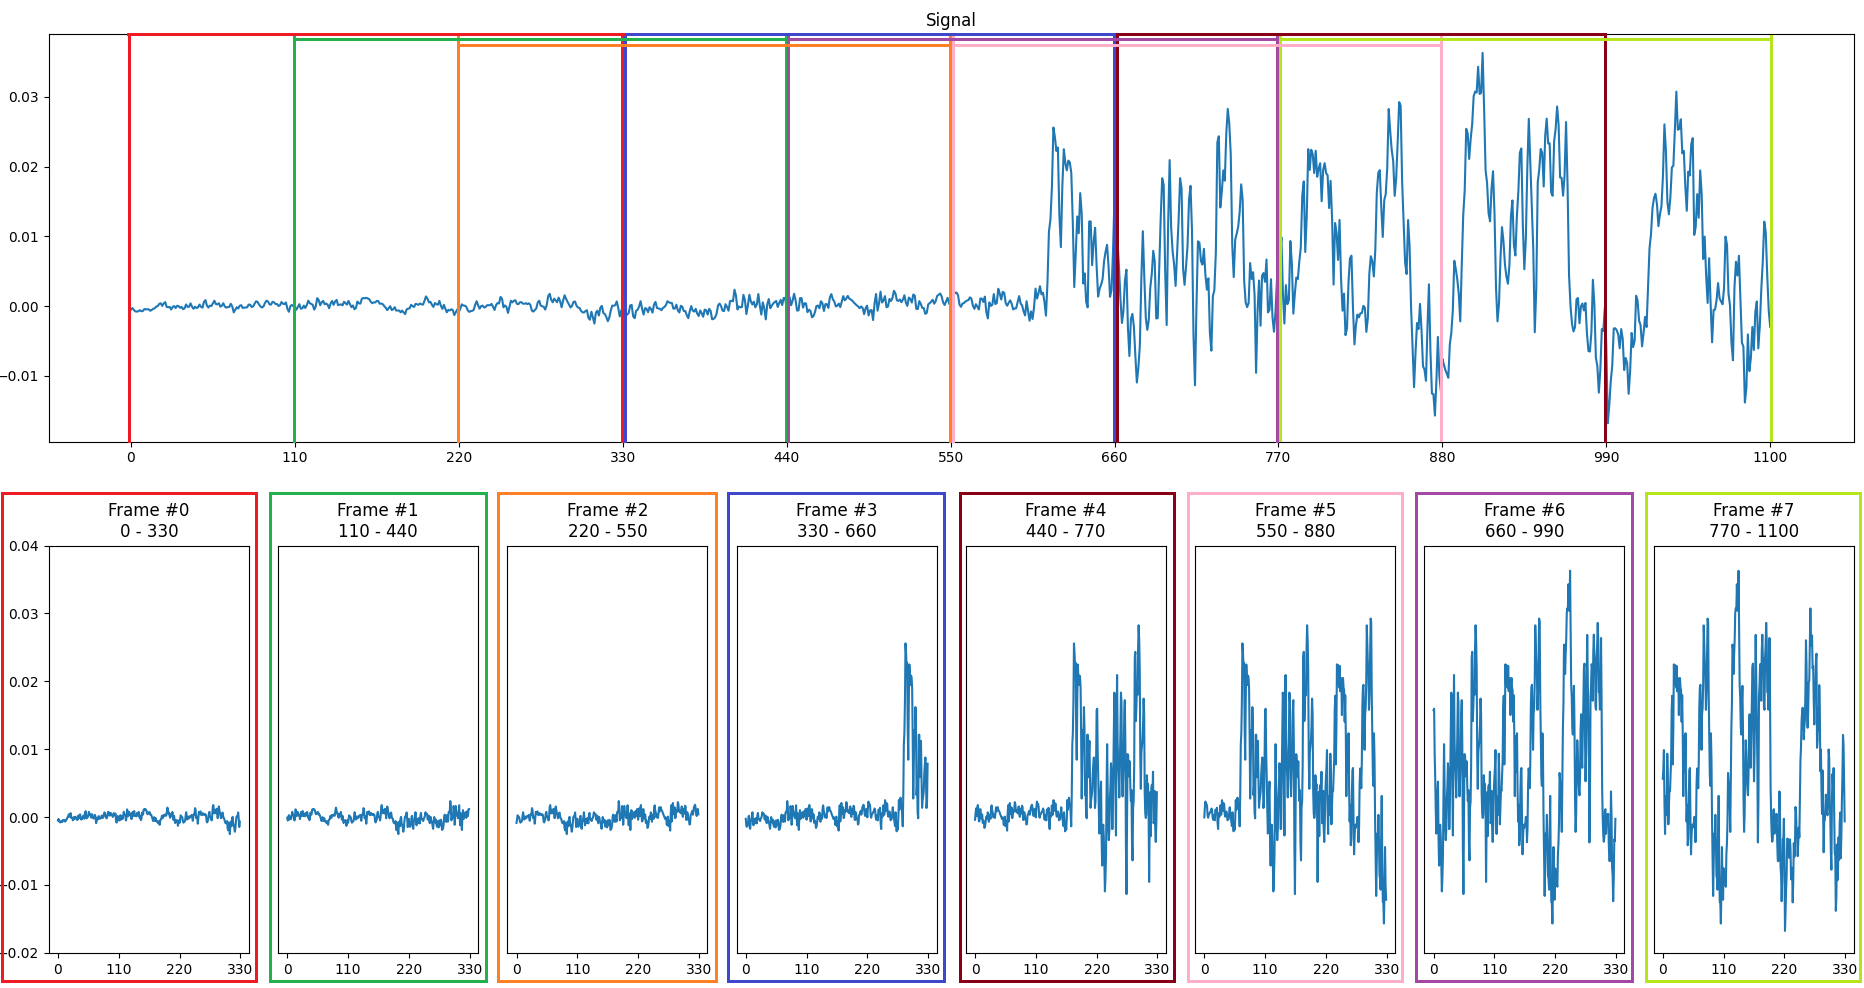
\includegraphics[width=\linewidth]{img/signal_framing.png}
\end{figure}

\subsubsection{Windowing}
Windowing involves applying a function to each frame to taper its edges, which minimizes a phenomenon known as spectral leakage. This effect occurs during the Discrete Fourier Transform (DFT), where the frequency components of a frame spread across multiple frequency bins, reducing the accuracy of spectral representation. Various window functions can be used, with the Hamming and Hann windows being among the most common in audio analysis. A rectangular window can also be applied, but it does not modify the signal, resulting in no reduction of spectral leakage\cite{hamid2018frame}. The Hamming and Hann windows differ in their behaviour at the boundaries: the Hann window tapers to zero at both ends, while the Hamming window retains small non-zero values (equal to 0.08 at the boundaries), resulting in less attenuation at the edges.
The window functions are defined as follows:
\begin{itemize}
  \item Hamming window
    \[
      w_{\text{Hamming}}[k]=0.54 - 0.46\cos{\left (\frac{2\pi k}{N-1}\right )}
    \]
  \item Hann window
    \[
      w_{\text{Hann}}[k]=0.5\cdot\Bigg(1-\cos{\left (\frac{2\pi k}{N-1}\right )\Bigg)}
    \]
  \item Rectangular window
    \[
      w_{\text{Rect}}[k]=1
    \]
\end{itemize}
where:
\begin{itemize}
  \item $N$ - window length
  \item $k$ - sample index
\end{itemize}

\begin{figure}[h]
  \caption{Window charts}
  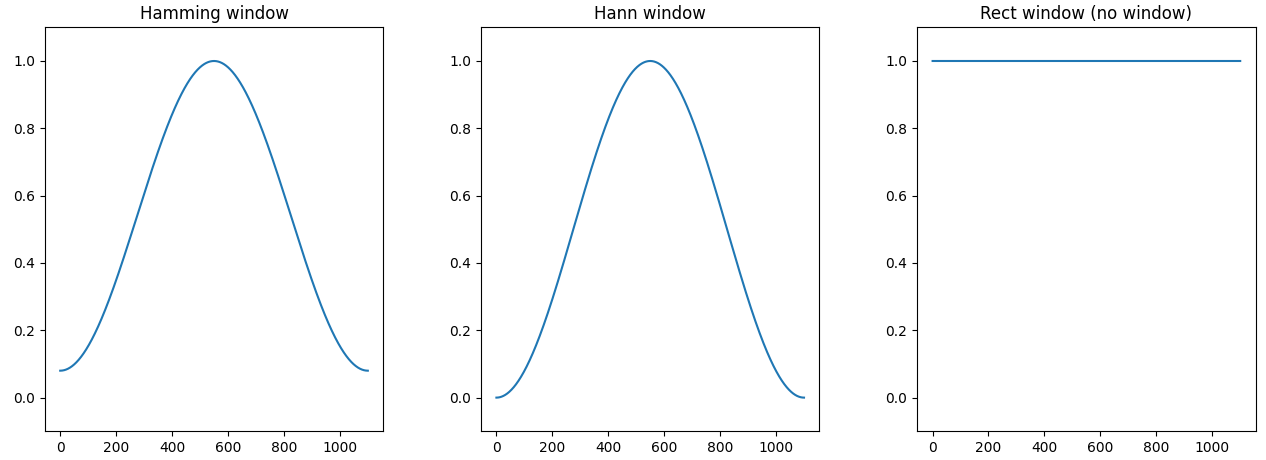
\includegraphics[width=\linewidth]{img/window_plots.png}
\end{figure}

\subsubsection{Transformation}

Audio analysis uses various mathematical transformation to convert time-domain audio into suitable representations for feature extraction (these representations are also suitable for visualization and manipulation)\cite{yustisar2020discrete,tzanetakis2001audio}. Experiments included in this paper focus on frequency domain transformation, specifically on Discrete Fourier Transform (DFT). It maps a signal frame to a set of amplitudes using the following formula:
\[
	A_k=\sum\limits_{p=0}^{n-1}a_ke^{-\dfrac{i2\pi kp}{n}}
\]
where:
\begin{itemize}
  \item $i$ - imaginary unit
  \item $k$ - frame index
  \item $n$ - sample count in frame $a$ (frame length)
  \item $a_k$ - sample at index $k$ in frame $a$
\end{itemize}

\subsubsection{Spectrum}

\subsubsection{Mel Filterbank}

\subsubsection{Mel Energies}

\subsubsection{Mel-Frequency Cepstral Coefficients}

\subsection{Machine Learning Algorithms}

\section{Experiments}
%Opis bazy

%Opis podziału, testów itd.


%Należy dodać wykresy, analizy i wszystko szczegółowo omówić - co widać na wykresach, %dlaczego itd.

\section{Conclusion}


%% Define the bibliography file to be used
\bibliography{bibliography}

\end{document}

%%
%% End of file
